%%%%%%%%%%%%%%%%%%%%%%%%%%%%%%%%%%%%%%%%%%%%%%%%%%%%%%%%%%%%%%%%%%%%%%%%%%%%%%%%
% VPIC Gordon Bell submission 2008
%
% $LastChangedRevision$
% $LastChangedDate$
% $LastChangedBy$
%
%%%%%%%%%%%%%%%%%%%%%%%%%%%%%%%%%%%%%%%%%%%%%%%%%%%%%%%%%%%%%%%%%%%%%%%%%%%%%%%%
\documentclass[letter,10pt]{article}

%%%%%%%%%%%%%%%%%%%%%%%%%%%%%%%%%%%%%%%%%%%%%%%%%%%%%%%%%%%%%%%%%%%%%%%%%%%%%%%%
% packages
%%%%%%%%%%%%%%%%%%%%%%%%%%%%%%%%%%%%%%%%%%%%%%%%%%%%%%%%%%%%%%%%%%%%%%%%%%%%%%%%
\usepackage{amsmath}
\usepackage{color}
\usepackage{latexmake}

%%%%%%%%%%%%%%%%%%%%%%%%%%%%%%%%%%%%%%%%%%%%%%%%%%%%%%%%%%%%%%%%%%%%%%%%%%%%%%%%
% add to document dimensions
% fudge if we need to add more space
%%%%%%%%%%%%%%%%%%%%%%%%%%%%%%%%%%%%%%%%%%%%%%%%%%%%%%%%%%%%%%%%%%%%%%%%%%%%%%%%
\addtolength{\topmargin}{-2cm}
\addtolength{\textheight}{3cm}
\addtolength{\oddsidemargin}{-2.25cm}
\addtolength{\evensidemargin}{-2.25cm}
\addtolength{\textwidth}{4.5cm}

%%%%%%%%%%%%%%%%%%%%%%%%%%%%%%%%%%%%%%%%%%%%%%%%%%%%%%%%%%%%%%%%%%%%%%%%%%%%%%%%
% article information
%%%%%%%%%%%%%%%%%%%%%%%%%%%%%%%%%%%%%%%%%%%%%%%%%%%%%%%%%%%%%%%%%%%%%%%%%%%%%%%%
\title{0.4 PFlop/s Trillion-Particle Particle-in-Cell Modeling of Laser Plasma Interactions on Roadrunner}
\author{%
B. Albright\thanks{Applied Physics Division (X-1-PTA Plasma Theory and Applications), Los Alamos National Laboratory, Los Alamos, NM 87544, Email: \emph{balbright@lanl.gov}} \and%
%
K. Barker\thanks{Computer, Computational, and Statistical Sciences Division (CCS-1 Computer Science on High Performance Computing), Los Alamos National Laboratory, Los Alamos, NM 87544, Email: \emph{kjbarker@lanl.gov}} \and%
%
B. Bergen\thanks{Computer, Computational, and Statistical Sciences Division (CCS-2 Computational Physics), Los Alamos National Laboratory, Los Alamos, NM 87544, Email: \emph{bergen@lanl.gov}} \and%
%
K. Bowers\thanks{D.E. Shaw Research LLC, 120 W 45th Street, 39th Floor, New York, NY 10036, Email: \emph{kevin.j.bowers@gmail.com}} \and%
%
D. Kerbyson\thanks{Computer, Computational, and Statistical Sciences Division (CCS-1 Computer Science on High Performance Computing), Los Alamos National Laboratory, Los Alamos, NM 87544, Email: \emph{djk@lanl.gov}} \and%
%
L. Yin\thanks{Applied Physics Division (X-1-PTA Plasma Theory and Applications), Los Alamos National Laboratory, Los Alamos, NM 87544, Email: \emph{lyin@lanl.gov}}}
\date{\today}

% if we have assessment, then we need to include CCS-1 types, no? 

%%%%%%%%%%%%%%%%%%%%%%%%%%%%%%%%%%%%%%%%%%%%%%%%%%%%%%%%%%%%%%%%%%%%%%%%%%%%%%%%
% begin document
%%%%%%%%%%%%%%%%%%%%%%%%%%%%%%%%%%%%%%%%%%%%%%%%%%%%%%%%%%%%%%%%%%%%%%%%%%%%%%%%
\begin{document}

%%%%%%%%%%%%%%%%%%%%%%%%%%%%%%%%%%%%%%%%%%%%%%%%%%%%%%%%%%%%%%%%%%%%%%%%%%%%%%%%
% title
%%%%%%%%%%%%%%%%%%%%%%%%%%%%%%%%%%%%%%%%%%%%%%%%%%%%%%%%%%%%%%%%%%%%%%%%%%%%%%%%
\maketitle
\thispagestyle{empty}

%%%%%%%%%%%%%%%%%%%%%%%%%%%%%%%%%%%%%%%%%%%%%%%%%%%%%%%%%%%%%%%%%%%%%%%%%%%%%%%%
% abstract
%%%%%%%%%%%%%%%%%%%%%%%%%%%%%%%%%%%%%%%%%%%%%%%%%%%%%%%%%%%%%%%%%%%%%%%%%%%%%%%%
\begin{abstract}
We demonstrate the outstanding performance and scalability of the VPIC kinetic plasma modeling code on the heterogeneous IBM Roadrunner supercomputer at Los Alamos National Laboratory.  VPIC is a three-dimensional, relativistic, electromagnetic, particle-in-cell code that self-consistently evolves a kinetic plasma.  VPIC simulations of laser plasma interaction (LPI) have been conducted at unprecedented fidelity and scale ---one trillion simulation macro particles on 125 million computational cells-- to accurately model the plasma environment inside a laser-driven hohlraum in an inertial confinement fusion experiment.   Sustained performance of approximately 0.4~Pflop/s was achieved.  This capability opens up the exciting possibility of using VPIC to model, in a first-principles manner, a problem that threatens the success of the multi-billion dollar DOE/NNSA National Ignition Facility.  
\end{abstract}

%%%%%%%%%%%%%%%%%%%%%%%%%%%%%%%%%%%%%%%%%%%%%%%%%%%%%%%%%%%%%%%%%%%%%%%%%%%%%%%%
% add break after title page
%%%%%%%%%%%%%%%%%%%%%%%%%%%%%%%%%%%%%%%%%%%%%%%%%%%%%%%%%%%%%%%%%%%%%%%%%%%%%%%%
\pagebreak

%%%%%%%%%%%%%%%%%%%%%%%%%%%%%%%%%%%%%%%%%%%%%%%%%%%%%%%%%%%%%%%%%%%%%%%%%%%%%%%%
% Introduction
%%%%%%%%%%%%%%%%%%%%%%%%%%%%%%%%%%%%%%%%%%%%%%%%%%%%%%%%%%%%%%%%%%%%%%%%%%%%%%%%
\section*{Introduction}

%%%%%%%%%%%%%%%%%%%%%%%%%%%%%%%%%%%%%%%%%%%%%%%%%%%%%%%%%%%%%%%%%%%%%%%%%%%%%%%%
% Architecture
%%%%%%%%%%%%%%%%%%%%%%%%%%%%%%%%%%%%%%%%%%%%%%%%%%%%%%%%%%%%%%%%%%%%%%%%%%%%%%%%
\section*{RoadRunner system architecture}

\begin{figure}
    \begin{center}
    \scalebox{0.3}{\input{system.pstex_t}}
    \caption{RoadRunner System Overview}
    \label{fig:system}
    \end{center}
\end{figure}

The RoadRunner supercomputer, shown in Figure \ref{fig:system}, is a hybrid, petascale system to be deployed at Los Alamos National Laboratory in 2008.  The system is a first-of-its-kind, heterogeneous cluster-of-clusters that utilizes a combination of 6,912 1.8 GHz, dual-socket, dual-core AMD Opteron \emph{host} processors with 12,960 3.2 GHz, IBM Cell \emph{extended Double-Precision (eDP)} \emph{accelerator} processors.  Each Cell eDP chip is capable of performing 102.4 Gflop/s \textbf{double-precision}, for a total theoretical peak performance of $\sim$1.3 Pflop/s\footnote{The Opteron base system has a theoretical peak performance of $\sim$50 Tflop/s.}.  The RoadRunner supercomputer will be the first machine to achieve a sustained petaflop on the LINPACK benchmark used in ranking the fastest supercomputers in the world for the TOP500 list \cite{top500}.

\subsection*{Connected Unit}

A Connected Unit (CU) is made up of 180 \emph{Triblade}, compute nodes and 12 I/O nodes linked by a first-stage, 288-port Voltaire Infiniband $4x$ DDR switch.  Using a top-down description, the system is comprised of 18 CUs, using eight, second-stage, 288-port Voltaire Infiniband $4x$ DDR switches.  This allows for twelve links per CU to each of the eight switches, with 192 ports \emph{in} and 96 ports \emph{up}, creating a 2-to-1 over-subscribed, fat-tree network topology.

A Connected Unit is a powerful cluster in its own right, with a theoretical peak performance of $\sim$74 Tflop/s.  A single CU of RoadRunner would rank in the top 20 on the current (November 2007) TOP500 list.

\begin{figure}
    \begin{center}
    \scalebox{0.4}{\input{triblade.pstex_t}}
    \caption{Triblade Compute Node}
    \label{fig:triblade}
    \end{center}
\end{figure}

\subsection*{Triblade}

A Triblade compute node, Figure \ref{fig:triblade}, actually integrates four physical blades: one IBM LS21, dual-socket Opteron blade, one expansion blade, and two IBM QS22 Cell blades containing the new eDP chips.  The expansion blade connects the two QS22s to the LS21 via four PCI-e $x8$ links and provides the node's ConnectX IB $4x$ DDR link to the rest of the CU cluster.  Each PCI-e $x8$ link logically connects an Opteron core to a Cell processor ---there is a one-to-one relationship between Opteron cores and Cell chips-- with a theoretical bandwidth of 2 GB/s.  Triblades are completely diskless, running from RAM disks with NFS and Panasas \cite{panasas} to the LS21 only.

The LS21 blade incorporates two dual-core AMD Opteron processors running at 1.8 GHz with 4 GB RAM per core.  Each LS21 has a theoretical peak of 14.4 Gflop/s in double precision.

Each QS22 blade has two enhanced Double Precision (eDP) IBM Cell processors ---the official product name is IBM PowerXCell 8I-- running at 3.2 GHz with 8 GB RAM so that each Cell chip has 4 GB RAM.  The two QS22 blades have an aggregate theoretical peak performance of 409.6 Gflop/s in double precision.

In total, each Triblade has 32 GB RAM, with 16 GB RAM on the LS21 blade and 16 GB RAM each per QS22 blade, so that each logical processor in a compute node has 4 GB RAM.  The total theoretical peak performance per Triblade is 424 Gflop/s in double precision.  The full RoadRunner machine has a total of 3240 Triblade compute nodes.

\subsection*{Cell Broadband Engine Architecture (CBEA)}

\begin{figure}
    \begin{center}
    \scalebox{0.5}{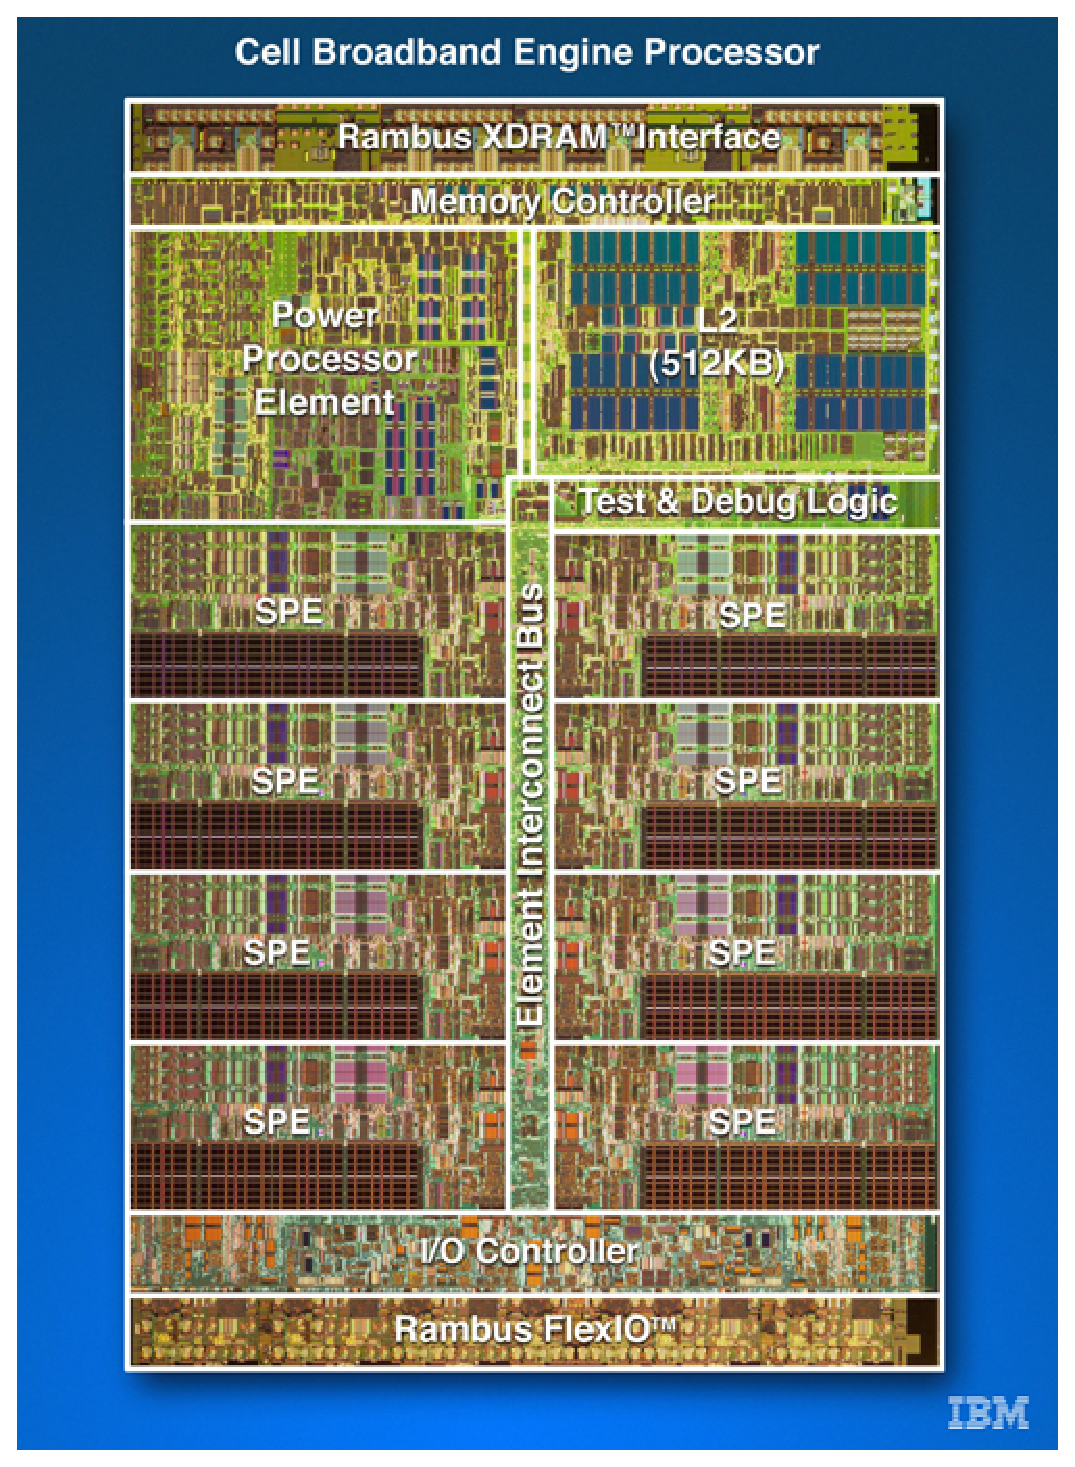
\includegraphics{cell}}
    \caption{Cell Broadband Engine}
    \label{image:cell}
    \end{center}
\end{figure}

The \emph{Cell Broadband Engine (Cell BE)}, developed jointly by Sony Computer Entertainment, Toshiba, and IBM, is an (8+1)-way, 90nm SOI, heterogeneous parallel processor that incorporates eight \emph{synergistic processing elements (SPEs)} and one \emph{power processing element (PPE)} connected via an \emph{Element Interconnect Bus (EIB)}.  The EIB also connects a memory controller (MIC) and two off-chip I/O interfaces.  This processor is used in the Sony Playstation 3 gaming console, and is currently offered in products from IBM (QS21 blade) and Mercury Computer Systems (CAB PCI-e card and DCBB2 blade) \cite{mercury}.

The PPE is a modestly provisioned general purpose processor capable of running the Linux OS, and which serves as a controller for the eight SPEs.  It supports two execution threads and has a theoretical peak performance of 6.4 Gflop/s double precision at 3.2 GHz.

Each SPE processor is a 128-bit vector engine with a 256 KB user-controlled, embedded SRAM called the \emph{Local Store (LS)}.  Additionally, each SPE has a 128-bit, 128-entry register file.  All data and text operated on by the SPE must be fetched from main memory to the LS using \emph{direct memory access (DMA)} calls.  Each SPE has its own \emph{Memory Flow Controller (MFC)} that supports up to 12 outstanding DMA requests and has a theoretical bandwidth of 25.6 GB/s to main memory using DDR2-800 SDRAM\footnote{The current plan of record for RoadRunner calls for DDR2-667, in which case, the theoretical bandwidth will be 21.4 GB/s.}.  SPEs support dual-issue on even and odd execution pipelines and have a theoretical single-precision, peak performance of 204.8 Gflop/s at 3.2 GHz.  Double-precision computation is possible on the Cell BE, although at the much lower rate of $\sim$14.63 Gflop/s at 3.2 GHz.

The EIB is configured as a four-way, circular ring with paired counter-rotating, uni-directional channels that are each 16 bytes wide.  There are currently 12 units connected to this bus, so that the maximum number of steps between any two units is six.  Each SPE has a 16 byte read port and a 16 byte write port, and is capable of performing a read or write of 16 bytes on every EIB clock cycle.  SPEs are able overlap computation with communication using special DMA queues for requests that are still in flight.  The EIB operates at one-half the system clock speed and has an aggregate theoretical bandwidth of 204.8 GB/s at 3.2 GHz.

\subsection*{IBM PowerXCell 8I (eDP)}

IBM has developed an enhanced version of the Cell BE chip specifically designed for use in supercomputing.  This chip, the IBM PowerXCell 8I, adds fully-pipelined, double-precision computing capability to the SPEs of the Cell BE chip.  The PowerXCell 8I uses a 65nm SOI process and has a double-precision theoretical peak performance of 102.4 Gflop/s at 3.2 GHz.  Except as regards double-precision performance, the PowerXCell 8I does not differ significantly from the Cell BE.  This is the Cell chip that is used in RoadRunner.

%%%%%%%%%%%%%%%%%%%%%%%%%%%%%%%%%%%%%%%%%%%%%%%%%%%%%%%%%%%%%%%%%%%%%%%%%%%%%%%%
% Science
%%%%%%%%%%%%%%%%%%%%%%%%%%%%%%%%%%%%%%%%%%%%%%%%%%%%%%%%%%%%%%%%%%%%%%%%%%%%%%%%
\section*{Inertial Confinement Fusion}

%%%%%%%%%%%%%%%%%%%%%%%%%%%%%%%%%%%%%%%%%%%%%%%%%%%%%%%%%%%%%%%%%%%%%%%%%%%%%%%%
% Science method
%%%%%%%%%%%%%%%%%%%%%%%%%%%%%%%%%%%%%%%%%%%%%%%%%%%%%%%%%%%%%%%%%%%%%%%%%%%%%%%%
\section*{Plasma Physics Simulations}

%%%%%%%%%%%%%%%%%%%%%%%%%%%%%%%%%%%%%%%%%%%%%%%%%%%%%%%%%%%%%%%%%%%%%%%%%%%%%%%%
% Numerical approach
%%%%%%%%%%%%%%%%%%%%%%%%%%%%%%%%%%%%%%%%%%%%%%%%%%%%%%%%%%%%%%%%%%%%%%%%%%%%%%%%
\section*{The VPIC Particle-In-Cell Code}

VPIC is a three-dimensional, relativistic, electromagnetic, particle-in-cell code that has been highly optimized to minimize data movement, a predominate consideration that must be addressed for many codes in order to achieve high levels of performance on modern computing architectures.  As a part of this strategy, VPIC uses an asymptotically optimal sorting algorithm to re-arrange particle data, at a compile-time configurable rate, to maintain good spatial locality of memory access to particle data.  This approach also increases temporal locality of the field data accesses used to update particle positions and velocities.  Additionally, the data layouts and computational algorithms used by VPIC have been designed to take advantage of the short-vector, SIMD execution pipelines that are available on many modern processors.  These characteristics, combined with VPIC's effective use of single-precision floating-point computation --- a factor of two increase in the theoretical peak attainable on some architectures, and a factor of two decrease in data movement --, make it one of the highest performing particle-in-cell applications in existence.

%%%%%%%%%%%%%%%%%%%%%%%%%%%%%%%%%%%%%%%%%%%%%%%%%%%%%%%%%%%%%%%%%%%%%%%%%%%%%%%%
% Moving the code to RoadRunner
%%%%%%%%%%%%%%%%%%%%%%%%%%%%%%%%%%%%%%%%%%%%%%%%%%%%%%%%%%%%%%%%%%%%%%%%%%%%%%%%
\section*{Adapting VPIC to RoadRunner}

\begin{figure}
    \begin{center}
    \scalebox{0.4}{\input{relay.pstex_t}}
    \caption{MP Relay}
    \label{fig:relay}
    \end{center}
\end{figure}

%%%%%%%%%%%%%%%%%%%%%%%%%%%%%%%%%%%%%%%%%%%%%%%%%%%%%%%%%%%%%%%%%%%%%%%%%%%%%%%%
% Performance and Scalability
%%%%%%%%%%%%%%%%%%%%%%%%%%%%%%%%%%%%%%%%%%%%%%%%%%%%%%%%%%%%%%%%%%%%%%%%%%%%%%%%
\section*{Performance and Scalability}

%%%%%%%%%%%%%%%%%%%%%%%%%%%%%%%%%%%%%%%%%%%%%%%%%%%%%%%%%%%%%%%%%%%%%%%%%%%%%%%%
% Conclusion
%%%%%%%%%%%%%%%%%%%%%%%%%%%%%%%%%%%%%%%%%%%%%%%%%%%%%%%%%%%%%%%%%%%%%%%%%%%%%%%%
\section*{Conclusion}

%%%%%%%%%%%%%%%%%%%%%%%%%%%%%%%%%%%%%%%%%%%%%%%%%%%%%%%%%%%%%%%%%%%%%%%%%%%%%%%%
% biliography
%%%%%%%%%%%%%%%%%%%%%%%%%%%%%%%%%%%%%%%%%%%%%%%%%%%%%%%%%%%%%%%%%%%%%%%%%%%%%%%%
\bibliographystyle{plain}
\bibliography{bib/gb2008,bib/vpic}

%%%%%%%%%%%%%%%%%%%%%%%%%%%%%%%%%%%%%%%%%%%%%%%%%%%%%%%%%%%%%%%%%%%%%%%%%%%%%%%%
% end document
%%%%%%%%%%%%%%%%%%%%%%%%%%%%%%%%%%%%%%%%%%%%%%%%%%%%%%%%%%%%%%%%%%%%%%%%%%%%%%%%
\end{document}
